\documentclass[10pt]{article}
\usepackage[polish]{babel}
\usepackage[utf8]{inputenc}
\usepackage[T1]{fontenc}
\usepackage{graphicx}
\usepackage[export]{adjustbox}
\graphicspath{ {./images/} }
\usepackage{amsmath}
\usepackage{amsfonts}
\usepackage{amssymb}
\usepackage[version=4]{mhchem}
\usepackage{stmaryrd}
\usepackage{hyperref}
\hypersetup{colorlinks=true, linkcolor=blue, filecolor=magenta, urlcolor=cyan,}
\urlstyle{same}
\usepackage{multirow}

\title{PRÓBNY EGZAMIN MATURALNY Z NOWĄ ERĄ MATEMATYKA - POZIOM ROZSZERZONY }

\author{}
\date{}


\newcommand\Varangle{\mathop{{<\!\!\!\!\!\text{\small)}}\:}\nolimits}

\begin{document}
\maketitle
KOD ZDAJĄCEGO\\
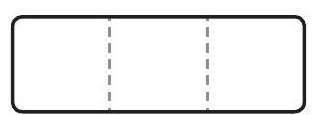
\includegraphics[max width=\textwidth, center]{2024_11_21_5abc0108fbbc287103ecg-01(1)}\\
symbol klasy\\
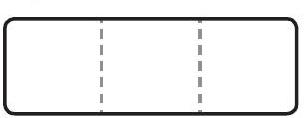
\includegraphics[max width=\textwidth, center]{2024_11_21_5abc0108fbbc287103ecg-01}\\
symbol zdającego

\section*{Instrukcja dla zdającego}
\begin{enumerate}
  \item Sprawdź, czy arkusz egzaminacyjny zawiera 20 stron (zadania 1-16). Ewentualny brak stron zgłoś nauczycielowi nadzorującemu egzamin.
  \item Rozwiązania zadań i odpowiedzi zapisz w miejscu na to przeznaczonym.
  \item Pamiętaj, że pominięcie argumentacji lub istotnych obliczeń w rozwiązaniu zadań otwartych może spowodować, że za to rozwiązanie nie otrzymasz pełnej liczby punktów.
  \item Pisz czytelnie. Używaj długopisu/pióra tylko z czarnym tuszem/atramentem.
  \item Nie używaj korektora, a błędne zapisy wyraźnie przekreśl.
  \item Pamiętaj, że zapisy w brudnopisie nie będą oceniane.
  \item Podczas egzaminu możesz korzystać z zestawu wzorów matematycznych, cyrkla i linijki oraz kalkulatora prostego.
  \item Na tej stronie wpisz swój kod.
  \item Nie wpisuj żadnych znaków w części przeznaczonej dla osoby sprawdzającej.
\end{enumerate}

Powodzenia!

\section*{\(\square\) \\
 dysleksja}
STYCZEŃ 2019

Czas pracy:\\
180 minut

Liczba punktów\\
do uzyskania: 50

W zadaniach 1.-4. wybierz izaznacz na karcie odpowiedzi poprawną odpowiedź.

\section*{Zadanie 1. (0-1)}
Liczba \(4^{\log _{2}\left(\frac{1}{\sqrt{2}-1}\right)}\) jest równa\\
A. \(\sqrt{2}+1\).\\
B. \(2+2 \sqrt{2}\).\\
C. \(3-2 \sqrt{2}\).\\
D. \(3+2 \sqrt{2}\).

\section*{Zadanie 2. (0-1)}
Liczba \(\frac{|x-|x||}{x}\) jest dla każdego \(x \neq 0\)\\
A. dodatnia.\\
B. nieujemna.\\
C. ujemna.\\
D. niedodatnia.

\section*{Zadanie 3. (0-1)}
Ciąg liczb rzeczywistych \(a_{1}, a_{2}, \ldots\) jest zdefiniowany warunkami \(a_{1}=1\) oraz \(\left(a_{n+1}\right)^{3}=99\left(a_{n}\right)^{3}\) dla \(n \geqslant 1\). Wówczas wyraz \(a_{100}\) jest równy\\
A. \(33^{33}\).\\
B. \(33^{99}\).\\
C. \(99^{33}\).\\
D. \(99^{99}\).

\section*{Zadanie 4. (0-1)}
Wskaż zbiór wszystkich rozwiązań równania \(|\cos (\alpha)+\cos (3 \alpha)+\cos (5 \alpha)|=3\).\\
A. \(\left\{\alpha: \alpha=n \cdot 60^{\circ}, n\right.\) jest dowolną liczbą całkowitą \(\}\)\\
B. \(\left\{\alpha: \alpha=n \cdot 90^{\circ}, n\right.\) jest dowolną liczbą całkowitą \(\}\)\\
C. \(\left\{\alpha: \alpha=n \cdot 180^{\circ}, n\right.\) jest dowolną liczbą całkowitą \(\}\)\\
D. \(\left\{\alpha: \alpha=n \cdot 360^{\circ}, n\right.\) jest dowolną liczbą całkowitą \(\}\)

\section*{Zadanie 5. (0-2)}
Oblicz granicę ciągu o wyrazie \(a_{n}=2(\sqrt{n+100 \sqrt{n}+5}-\sqrt{n-\sqrt{n}+200})\).\\
W poniższe kratki wpisz kolejno cyfry wyniku.\\
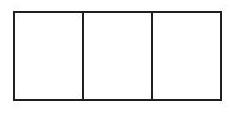
\includegraphics[max width=\textwidth, center]{2024_11_21_5abc0108fbbc287103ecg-02}

\section*{BRUDNOPIS (nie podlega ocenie)}
Więcej arkuszy znajdziesz na stronie: \href{http://arkusze.pl}{arkusze.pl}\\

\includegraphics[max width=\textwidth, center]{2024_11_21_5abc0108fbbc287103ecg-03}

\begin{center}
\begin{tabular}{|l|l|c|c|c|c|c|}
\hline
\multirow{2}{*}{\begin{tabular}{c}
Wypełnia \\
sprawdzający \\
\end{tabular}} & Nr zadania & 1 & 2 & 3 & 4 & 5 \\
\cline { 2 - 7 }
 & Maks. liczba pkt & 1 & 1 & 1 & 1 & 2 \\
\cline { 2 - 7 }
 & Uzyskana liczba pkt &  &  &  &  &  \\
\hline
\end{tabular}
\end{center}

Zadanie 6. (0-2)\\
Wyznacz parę liczb \(p, q \in R\) tak, by wielomian \(x^{4}+p x^{2}+q\) był podzielny przez trójmian \(x^{2}+6 x+5\).

Więcej arkuszy znajdziesz na stronie: \href{http://arkusze.pl}{arkusze.pl}\\

\includegraphics[max width=\textwidth, center]{2024_11_21_5abc0108fbbc287103ecg-04}

Odpowiedź:

\section*{Zadanie 7. (0-2)}
Wyznacz liczbę takich permutacji zbioru \(\{1,2,3, \ldots, 31\}\) kolejnych liczb całkowitych z przedziału \(\langle 1,31\rangle\), w których iloczyn każdych dwóch sąsiednich liczb jest liczbą parzystą. Wynik przedstaw w postaci iloczynu \(m!\cdot n\) !, gdzie \(m, n\) są pewnymi liczbami całkowitymi.\\

\includegraphics[max width=\textwidth, center]{2024_11_21_5abc0108fbbc287103ecg-05}

Odpowiedź:

\begin{center}
\begin{tabular}{|l|l|c|c|}
\hline
\multirow{2}{*}{\begin{tabular}{c}
Wypełnia \\
sprawdzający \\
\end{tabular}} & Nr zadania & 6 & 7 \\
\cline { 2 - 4 }
 & Maks. liczba pkt & 2 & 2 \\
\cline { 2 - 4 }
 & Uzyskana liczba pkt &  &  \\
\hline
\end{tabular}
\end{center}

Zadanie 8. (0-3)\\
Długości boków czworokąta wypukłego \(A B C D\) wynoszą: \(|A B|=a,|B C|=2 a,|C D|=b,|A D|=2 b\). Wykaż, że jeśli pole czworokąta \(A B C D\) jest równe \(a^{2}+b^{2}\), to jest on prostokątem.

Więcej arkuszy znajdziesz na stronie: \href{http://arkusze.pl}{arkusze.pl}\\

\includegraphics[max width=\textwidth, center]{2024_11_21_5abc0108fbbc287103ecg-06}

Zadanie 9. (0-3)\\
Dany jest trapez \(A B C D\), w którym kąty \(A B C\) i \(B C D\) są proste, \(|\Varangle D A B|=60^{\circ},|A B|=2\) oraz \(|B D|=\sqrt{3}\). Wyznacz długość odcinka \(A C\).\\

\includegraphics[max width=\textwidth, center]{2024_11_21_5abc0108fbbc287103ecg-07}

Odpowiedź:

\begin{center}
\begin{tabular}{|l|l|c|c|}
\hline
\multirow{2}{*}{\begin{tabular}{c}
Wypełnia \\
sprawdzający \\
\end{tabular}} & Nr zadania & 8 & 9 \\
\cline { 2 - 4 }
 & Maks. liczba pkt & 3 & 3 \\
\cline { 2 - 4 }
 & Uzyskana liczba pkt &  &  \\
\hline
\end{tabular}
\end{center}

Zadanie 10. (0-3)\\
W pudełku znajduje się sto kul ponumerowanych liczbami od 1 do 100. Wylosowanie każdej z kul jest tak samo prawdopodobne. Wylosowano jednocześnie pięć kul. Wyznacz prawdopodobieństwo, że numery wylosowanych kul ustawione w odpowiedniej kolejności tworzą ściśle rosnący ciąg geometryczny o całkowitym ilorazie.\\

\includegraphics[max width=\textwidth, center]{2024_11_21_5abc0108fbbc287103ecg-08}

Odpowiedź:

Zadanie 11. (0-4)\\
Wykaż, że jeśli \(\alpha, \beta, \gamma\) są kątami trójkąta i zachodzi równość \(\frac{\sin ^{2} \alpha}{\sin ^{2} \beta}=\frac{\operatorname{tg} \alpha}{\operatorname{tg} \beta}\), to \(\alpha=\beta\) lub \(\gamma=90^{\circ}\).

Więcej arkuszy znajdziesz na stronie: \href{http://arkusze.pl}{arkusze.pl}\\

\includegraphics[max width=\textwidth, center]{2024_11_21_5abc0108fbbc287103ecg-09}

\begin{center}
\begin{tabular}{|l|l|c|c|}
\hline
\multirow{2}{*}{\begin{tabular}{c}
Wypełnia \\
sprawdzający \\
\end{tabular}} & Nr zadania & 10 & 11 \\
\cline { 2 - 4 }
 & Maks. liczba pkt & 3 & 4 \\
\cline { 2 - 4 }
 & Uzyskana liczba pkt &  &  \\
\hline
\end{tabular}
\end{center}

Zadanie 12. (0-4)\\
Jednokładność \(f\) o środku w punkcie \(X\) przekształca punkt \(A=(3,2)\) na punkt \(A^{\prime}=(4,6)\) oraz przeprowadza punkt \(B=(-3,3)\) na punkt \(B^{\prime}=(-8,8)\). Znajdź równanie okręgu, którego obrazem przy jednokładności \(f\) jest okrąg o równaniu \((x-8)^{2}+(y-2)^{2}=4\).

Więcej arkuszy znajdziesz na stronie: \href{http://arkusze.pl}{arkusze.pl}\\

\includegraphics[max width=\textwidth, center]{2024_11_21_5abc0108fbbc287103ecg-10}\\
Więcej arkuszy znajdziesz na stronie: \href{http://arkusze.pl}{arkusze.pl}\\

\includegraphics[max width=\textwidth, center]{2024_11_21_5abc0108fbbc287103ecg-11}\\
Odpowiedź:

\begin{center}
\begin{tabular}{|l|l|c|}
\hline
\multirow{2}{*}{\begin{tabular}{c}
Wypełnia \\
sprawdzający \\
\end{tabular}} & Nr zadania & 12 \\
\cline { 2 - 3 }
 & Maks. liczba pkt & 4 \\
\cline { 2 - 3 }
 & Uzyskana liczba pkt &  \\
\hline
\end{tabular}
\end{center}

Zadanie 13. (0-5)\\
Wyznacz wszystkie wartości parametru \(m \in R\), dla których równanie \((1-m) 9^{x}+4 \cdot 3^{x}=m+2\) ma dwa różne rozwiązania rzeczywiste.\\

\includegraphics[max width=\textwidth, center]{2024_11_21_5abc0108fbbc287103ecg-12}\\
Więcej arkuszy znajdziesz na stronie: \href{http://arkusze.pl}{arkusze.pl}\\

\includegraphics[max width=\textwidth, center]{2024_11_21_5abc0108fbbc287103ecg-13}\\
Odpowiedź:

\begin{center}
\begin{tabular}{|l|l|c|}
\hline
\multirow{3}{*}{\begin{tabular}{c}
Wypełnia \\
sprawdzający \\
\end{tabular}} & Nr zadania & 13 \\
\cline { 2 - 3 }
 & Maks. liczba pkt & 5 \\
\cline { 2 - 3 }
 & Uzyskana liczba pkt &  \\
\hline
\end{tabular}
\end{center}

Zadanie 14. (0-5)\\
Dany jest trójkąt \(A B C\) o polu równym 5, gdzie \(A=(5,3)\) oraz \(B=(1,0)\). Prosta zawierająca wysokość trójkąta \(A B C\) ma równanie \(y=2 x-7\). Wyznacz współrzędne punktu \(C\).\\

\includegraphics[max width=\textwidth, center]{2024_11_21_5abc0108fbbc287103ecg-14}\\
Więcej arkuszy znajdziesz na stronie: \href{http://arkusze.pl}{arkusze.pl}\\

\includegraphics[max width=\textwidth, center]{2024_11_21_5abc0108fbbc287103ecg-15}\\
Odpowiedź:

\begin{center}
\begin{tabular}{|l|l|c|}
\hline
\multirow{3}{*}{\begin{tabular}{c}
Wypełnia \\
sprawdzający \\
\end{tabular}} & Nr zadania & 14 \\
\cline { 2 - 3 }
 & Maks. liczba pkt & 5 \\
\cline { 2 - 3 }
 & Uzyskana liczba pkt &  \\
\hline
\end{tabular}
\end{center}

Zadanie 15. (0-6)\\
Para liczb \(\left(m_{0}, n_{0}\right)\) jest rozwiązaniem układu równań \(\left\{\begin{array}{l}m+n=2 \\ m-n=\frac{-2}{p+1}\end{array}\right.\), gdzie \(p \neq-1\).\\
a) Wyznacz wzór funkcji \(f(p)=\frac{m_{0}}{n_{0}}\), podaj jej dziedzinę i zbiór wartości.\\
b) Napisz równanie stycznej do wykresu funkcji \(f\) w punkcie \(P(-3, f(-3))\).

Więcej arkuszy znajdziesz na stronie: \href{http://arkusze.pl}{arkusze.pl}\\

\includegraphics[max width=\textwidth, center]{2024_11_21_5abc0108fbbc287103ecg-16}\\
Więcej arkuszy znajdziesz na stronie: \href{http://arkusze.pl}{arkusze.pl}\\

\includegraphics[max width=\textwidth, center]{2024_11_21_5abc0108fbbc287103ecg-17}\\
Odpowiedź:

\begin{center}
\begin{tabular}{|l|l|c|}
\hline
\multirow{3}{*}{\begin{tabular}{c}
Wypełnia \\
sprawdzający \\
\end{tabular}} & Nr zadania & 15 \\
\cline { 2 - 3 }
 & Maks. liczba pkt & 6 \\
\cline { 2 - 3 }
 & Uzyskana liczba pkt &  \\
\hline
\end{tabular}
\end{center}

Zadanie 16. (0-7)\\
Niech \(x\) będzie liczbą dodatnią. Rozpatrujemy wszystkie prostopadłościany spełniające następujące warunki:\\
(1) podstawą prostopadłościanu jest kwadrat o boku długości \(x\),\\
(2) pole (prostokątnego) przekroju prostopadłościanu płaszczyzną zawierającą krawędź podstawy i przekątne dwu ścian bocznych jest równe \(\sqrt{3}\) (patrz rysunek).

Zapisz kwadrat objętości tego prostopadłościanu jako funkcję zmiennej \(x\).\\
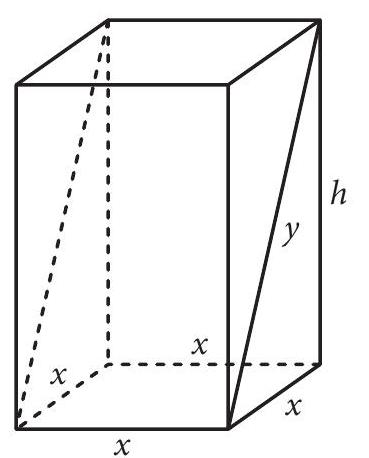
\includegraphics[max width=\textwidth, center]{2024_11_21_5abc0108fbbc287103ecg-18}

Wyznacz wszystkie wartości \(x>0\), dla których istnieje prostopadłościan spełniający drugi warunek.\\
Znajdź długości krawędzi tego spośród rozpatrywanych prostopadłościanów, którego objętość jest największa.

Więcej arkuszy znajdziesz na stronie: \href{http://arkusze.pl}{arkusze.pl}

\begin{center}
\begin{tabular}{|c|c|c|c|c|c|c|c|c|c|c|c|c|c|c|c|c|c|c|c|c|c|c|c|c|c|c|c|c|c|}
\hline
 &  &  &  &  &  &  &  &  &  &  &  &  &  &  &  &  &  &  &  &  &  &  &  &  &  &  &  &  &  \\
\hline
 &  &  &  &  &  &  &  &  &  &  &  &  &  &  &  &  &  &  &  &  &  &  &  &  &  &  &  &  &  \\
\hline
 &  &  &  &  &  &  &  &  &  &  &  &  &  &  &  &  &  &  &  &  &  &  &  &  &  &  &  &  &  \\
\hline
 &  &  &  &  &  &  &  &  &  &  &  &  &  &  &  &  &  &  &  &  &  &  &  &  &  &  &  &  &  \\
\hline
 &  &  &  &  &  &  &  &  &  &  &  &  &  &  &  &  &  &  &  &  &  &  &  &  &  &  &  &  &  \\
\hline
 &  &  &  &  &  &  &  &  &  &  &  &  &  &  &  &  &  &  &  &  &  &  &  &  &  &  &  &  &  \\
\hline
 &  &  &  &  &  &  &  &  &  &  &  &  &  &  &  &  &  &  &  &  &  &  &  &  &  &  &  &  &  \\
\hline
 &  &  &  &  &  &  &  &  &  &  &  &  &  &  &  &  &  &  &  &  &  &  &  &  &  &  &  &  &  \\
\hline
 &  &  &  &  &  &  &  &  &  &  &  &  &  &  &  &  &  &  &  &  &  &  &  &  &  &  &  &  &  \\
\hline
 &  &  &  &  &  &  &  &  &  &  &  &  &  &  &  &  &  &  &  &  &  &  &  &  &  &  &  &  &  \\
\hline
 &  &  &  &  &  &  &  &  &  &  &  &  &  &  &  &  &  &  &  &  &  &  &  &  &  &  &  &  &  \\
\hline
 &  &  &  &  &  &  &  &  &  &  &  &  &  &  &  &  &  &  &  &  &  &  &  &  &  &  &  &  &  \\
\hline
 &  &  &  &  &  &  &  &  &  &  &  &  &  &  &  &  &  &  &  &  &  &  &  &  &  &  &  &  &  \\
\hline
 &  &  &  &  &  &  &  &  &  &  &  &  &  &  &  &  &  &  &  &  &  &  &  &  &  &  &  &  &  \\
\hline
 &  &  &  &  &  &  &  &  &  &  &  &  &  &  &  &  &  &  &  &  &  &  &  &  &  &  &  &  &  \\
\hline
 &  &  &  &  &  &  &  &  &  &  &  &  &  &  &  &  &  &  &  &  &  &  &  &  &  &  &  &  &  \\
\hline
 &  &  &  &  &  &  &  &  &  &  &  &  &  &  &  &  &  &  &  &  &  &  &  &  &  &  &  &  &  \\
\hline
 &  &  &  &  &  &  &  &  &  &  &  &  &  &  &  &  &  &  &  &  &  &  &  &  &  &  &  &  &  \\
\hline
 &  &  &  &  &  &  &  &  &  &  &  &  &  &  &  &  &  &  &  &  &  &  &  &  &  &  &  &  &  \\
\hline
 &  &  &  &  &  &  &  &  &  &  &  &  &  &  &  &  &  &  &  &  &  &  &  &  &  &  &  &  &  \\
\hline
 &  &  &  &  &  &  &  &  &  &  &  &  &  &  &  &  &  &  &  &  &  &  &  &  &  &  &  &  &  \\
\hline
 &  &  &  &  &  &  &  &  &  &  &  &  &  &  &  &  &  &  &  &  &  &  &  &  &  &  &  &  &  \\
\hline
 &  &  &  &  &  &  &  &  &  &  &  &  &  &  &  &  &  &  &  &  &  &  &  &  &  &  &  &  &  \\
\hline
 &  &  &  &  &  &  &  &  &  &  &  &  &  &  &  &  &  &  &  &  &  &  &  &  &  &  &  &  &  \\
\hline
 &  &  &  &  &  &  &  &  &  &  &  &  &  &  &  &  &  &  &  &  &  &  &  &  &  &  &  &  &  \\
\hline
 &  &  &  &  &  &  &  &  &  &  &  &  &  &  &  &  &  &  &  &  &  &  &  &  &  &  &  &  &  \\
\hline
 &  &  &  &  &  &  &  &  &  &  &  &  &  &  &  &  &  &  &  &  &  &  &  &  &  &  &  &  &  \\
\hline
 &  &  &  &  &  &  &  &  &  &  &  &  &  &  &  &  &  &  &  &  &  &  &  &  &  &  &  &  &  \\
\hline
 &  &  &  &  &  &  &  &  &  &  &  &  &  &  &  &  &  &  &  &  &  &  &  &  &  &  &  &  &  \\
\hline
 &  &  &  &  &  &  &  &  &  &  &  &  &  &  &  &  &  &  &  &  &  &  &  &  &  &  &  &  &  \\
\hline
 &  &  &  &  &  &  &  &  &  &  &  &  &  &  &  &  &  &  &  &  &  &  &  &  &  &  &  &  &  \\
\hline
 &  &  &  &  &  &  &  &  &  &  &  &  &  &  &  &  &  &  &  &  &  &  &  &  &  &  &  &  &  \\
\hline
 &  &  &  &  &  &  &  &  &  &  &  &  &  &  &  &  &  &  &  &  &  &  &  &  &  &  &  &  &  \\
\hline
\end{tabular}
\end{center}

Więcej arkuszy znajdziesz na stronie: \href{http://arkusze.pl}{arkusze.pl}\\

\includegraphics[max width=\textwidth, center]{2024_11_21_5abc0108fbbc287103ecg-19}\\
Odpowiedź:

\begin{center}
\begin{tabular}{|l|l|c|}
\hline
\multirow{3}{*}{\begin{tabular}{c}
Wypełnia \\
sprawdzający \\
\end{tabular}} & Nr zadania & 16 \\
\cline { 2 - 3 }
 & Maks. liczba pkt & 7 \\
\cline { 2 - 3 }
 & Uzyskana liczba pkt &  \\
\hline
\end{tabular}
\end{center}

\section*{BRUDNOPIS (nie podlega ocenie)}
Więcej arkuszy znajdziesz na stronie: \href{http://arkusze.pl}{arkusze.pl}\\

\includegraphics[max width=\textwidth, center]{2024_11_21_5abc0108fbbc287103ecg-20}


\end{document}